\documentclass[
tikz,
border=5pt,
convert={density=600,
	outext=.png
	}
]{standalone}


\usepackage[utf8]{inputenc}
%\usepackage{/home/ccaprani/projects/Tikz-StructuralAnalysis/stanli.sty}
\usepackage{stanli}
\usepackage{tikz}
\usetikzlibrary{arrows.meta,arrows,positioning,calc,backgrounds}

\begin{document}
	
	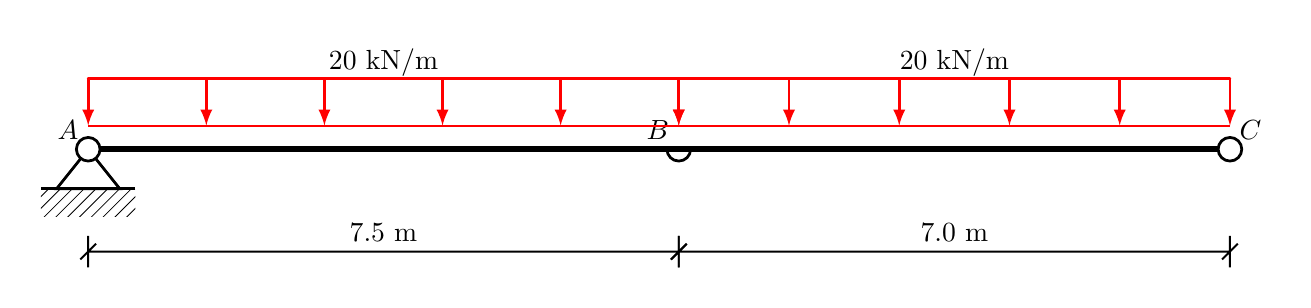
\begin{tikzpicture}[background rectangle/.style={fill=white!45}, show background rectangle]
		
		% Draw beam, supports, notation
		% Stations
		\point{a}{0}{0};
		\point{b}{7.5}{0};
		\point{c}{14.5}{0};
		
		% Midpoints for later reference
		\node (ab) at ($(a)!.5!(b)$) {};
		\node (bc) at ($(b)!.5!(c)$) {};
		
		% Draw the beam between the stations
		\foreach \startn/\endn in {a/b,b/c}
		\beam{4}{\startn}{\endn};
		
		% Supports
		\support{1}{a};
		\support{2ooo}{b};
		\support{2ooo}{c};
	 	\hinge{2}{b}[a][c];
		
		% hinges
		\foreach \startpt in {a,c}
			\hinge{1}{\startpt};
		
		% Dimensions
		\dimensioning{1}{a}{b}{-1.3}[$7.5$~m];
		\dimensioning{1}{b}{c}{-1.3}[$7.0$~m];
		
		% Letters - no ticks = 1; ticks = 2
		\notation {1}{a}{$A$}[above left];
		\notation {1}{b}{$B$}[above left];
		\notation {1}{c}{$C$}[above right];
		
		\begin{scope}[color=red]
			\lineload{1}{a}{b}[0.6][0.6];
			\lineload{1}{b}{c}[0.6][0.6];
		\end{scope}
		\notation{5}{a}{b}[$20$ kN/m][0.5][above=8mm];
		\notation{5}{b}{c}[$20$ kN/m][0.5][above=8mm];

	\end{tikzpicture}

\end{document}